\documentclass{beamer}
%\documentclass[handout]{beamer}

% language settings
%\usepackage{fontspec, polyglossia}
%\setdefaultlanguage{magyar}

% common packages
\usepackage{amsmath, multimedia, hyperref, color, multirow}
%\usepackage{graphicx}

% TikZ
\usepackage{tikz}
%\usetikzlibrary{arrows.meta, decorations.pathmorphing, decorations.pathreplacing, shapes.geometric,mindmap}
%\usetikzlibrary{shapes.geometric,fadings,bayesnet}

% beamer styles
\mode<presentation>{
\usetheme{Boadilla}
%\usetheme{Antibes}
%\usecolortheme{beaver}
%\usecolortheme{seahorse}
%\usefonttheme{structureitalicserif}
\setbeamercovered{transparent}
}
\setbeamertemplate{blocks}[rounded][shadow=true]
\AtBeginSubsection[]{
  \begin{frame}<beamer>{Contents}
    \tableofcontents[currentsection,currentsubsection]
  \end{frame}
}
%\useoutertheme[]{tree}

% title, etc
\title{The ``Imprinting Manuscript''}
\subtitle{Normal Expression Bias of Imprinted Genes in Schizophrenics}
\author{Attila Gulyas-Kovacs}
\date{Chess lab meeting 12/12/17}

\begin{document}

\maketitle

\begin{frame}[label=cmc]{The CommonMind data}
\includegraphics[width=1.0\textwidth]{figures/by-me/commonmind-rna-seq/commonmind-rna-seq.pdf}
\end{frame}

\begin{frame}
\begin{itemize}
\item questions
\begin{enumerate}
\item schizophrenia and imprinting (15q11-q13 microduplications)
\item imprinted genes in adult human DLPFC
\item determinants of imprinting (age, ancestry, gender)
\end{enumerate}
\item key studies
\begin{enumerate}
\item Gregg et al 2010 Science
\item Fromer et al 2016 Nat Neurosci
\item Baran et al 2015 Genome Res
\end{enumerate}
\end{itemize}
\end{frame}

\begin{frame}{\emph{Read count ratio} gauges \emph{allelic bias} and thus \emph{imprinting}}
\includegraphics[width=1.0\textwidth]{figures/by-me/commonmind-rna-seq-ms/commonmind-rna-seq-ms.pdf}
\end{frame}

\begin{frame}{Ranking genes based on variation across individuals}
\includegraphics[height=0.85\textheight]{figures/2016-07-19-genome-wide-S/complex-plot-1.png}
\end{frame}

\begin{frame}{Gene score and previous imprinted gene clusters}
\includegraphics[height=0.85\textheight]{figures/2016-08-08-imprinted-gene-clusters/score-genomic-location-1.png}
\end{frame}

\begin{frame}{Establishing imprinting status in the human DLPFC}
\begin{columns}[t]
\begin{column}{0.5\textwidth}
\begin{itemize}
\item prior expectation: near cluster
\item alternative causes of high read count ratio
\begin{enumerate}
\item mapping bias
\item eQTL
\end{enumerate}
\end{itemize}
\end{column}
\begin{column}{0.5\textwidth}

\includegraphics[height=0.85\textheight]{figures/2016-08-01-ifats-filters/top-ranking-genes-1.pdf}
\end{column}
\end{columns}
\end{frame}

\begin{frame}{Including 3 slightly lower scoring genes}
\includegraphics[height=0.85\textheight]{figures/2016-08-01-ifats-filters/known-genes-1.pdf}
\end{frame}

\begin{frame}{The imprinted genes and SCZ: marginal distribution}
\includegraphics[height=0.85\textheight]{figures/2016-11-01-plotting-distribution-of-s/S-Dx-strip-1.pdf}
\end{frame}

\begin{frame}{Why marginal distributions are misleading: dependencies}
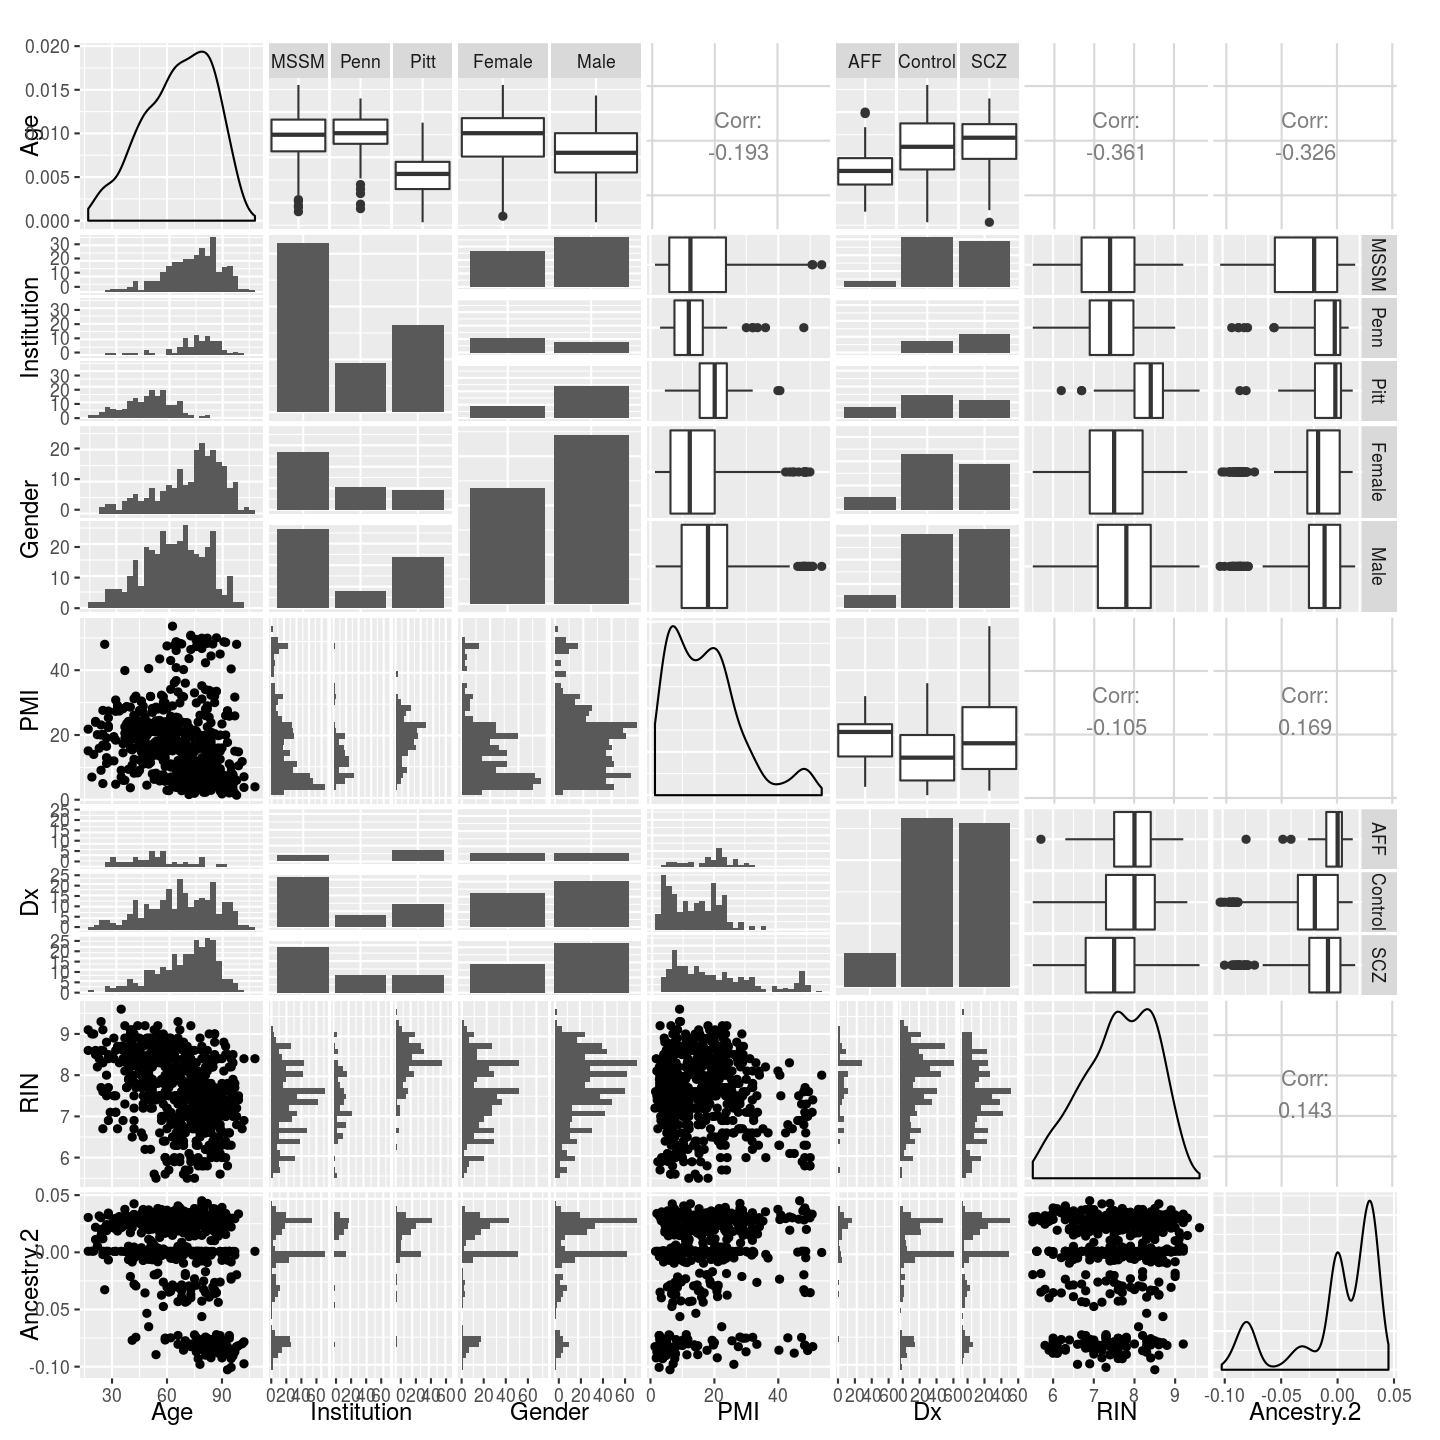
\includegraphics[height=0.85\textheight]{figures/2016-06-26-trellis-display-of-data/evar-scatterplot-matrix-2.png}
\end{frame}

\begin{frame}{Explanatory variables of read count ratio}
\begin{table}[H]
\begin{center}
\begin{tabular}{r|l}
explanatory variable & levels\\
\hline
Age &  \\
Institution & [MSSM], Penn, Pitt\\
Gender & [Female], Male\\
PMI & \\
Dx & [Control], SCZ, AFF \\
RIN &  \\
RNA\_batch & [A], B, C, D, E, F, G, H, 0\\
Ancestry.1 & \\
\vdots & \\
Ancestry.5 &  \\
\end{tabular}
\end{center}
\end{table}

\end{frame}

\end{document}



\begin{columns}[t]
\begin{column}{0.5\textwidth}

\end{column}

\begin{column}{0.5\textwidth}

\end{column}
\end{columns}
